\section{Cayley and the Algebra of Geometry: From Surfaces to Structure}

\subsection{The Leap from Jacobi to Cayley}

If Jacobi showed that motion could be described by sweeping surfaces in configuration space,  
then Arthur Cayley turned geometry itself into an algebra—  
an algebra not merely of points and curves, but of the very transformations that connected them.

Jacobi had taken Hamilton’s flow and reframed it as a problem of finding a special function \( S(q,t) \),  
whose gradients traced out every possible trajectory.  
In Jacobi’s hands, mechanics became a geometry of surfaces.

But Cayley asked a deeper question:

\begin{quote}
What lies behind the geometry of those surfaces themselves?
\end{quote}

Could geometry itself be reduced to operations?  
Could distance, angle, and curvature be encoded not in the figures drawn, but in the algebra of relations among them?

Jacobi’s Hamilton–Jacobi equation transformed mechanics into a problem of finding level sets in a function space.  
Each trajectory became a path along such a surface.

But Cayley saw geometry not as a study of shapes on a backdrop,  
but as a study of the algebraic relationships that defined the backdrop itself.

Where Jacobi worked with differential equations to describe curves,  
Cayley introduced matrices to describe transformations.

He realized that many geometric properties could be expressed through systems of equations—  
and that those systems could be represented, manipulated, and studied through arrays of numbers.

Thus was born the algebra of matrices.


In a world where Euclid had given us points and lines,  
and where Hamilton and Jacobi had given us flows and surfaces,  
Cayley gave us a way to describe transformations between spaces algebraically.

He introduced the \textbf{matrix product}, the \textbf{determinant}, and the notion of an abstract algebraic structure  
where geometry and linear transformations were two faces of the same coin.

\begin{HistoricalSidebar}{Cayley: Abstraction in the Shadow of Empire}

Arthur Cayley’s mathematical work reads like pure intellectual art: group theory, invariant theory, 
algebraic geometry, and the creation of matrix algebra. He was not building artillery tables, 
navigation charts, or celestial models. Instead, Cayley pursued mathematics for its internal 
structure — an abstract universe of symmetries, transformations, and algebraic relations.

\medskip

And yet, his ability to do so was entirely dependent on his time and place: the economic and political 
stability of the British Empire. Unlike many of his continental contemporaries, Cayley worked in a 
system where empire-funded universities, imperial trade wealth, and a global professional class provided 
both financial security and cultural space for "pure" research.

\medskip

By the mid-19th century, British science faced a prestige race against the rising rigor of German 
mathematics. While France and Germany tied mathematics tightly to state bureaucracy and military 
science, British elites sought to elevate pure mathematics as a marker of refined intellectual 
civilization — an empire that could afford to sponsor knowledge untethered from immediate utility.

\medskip

Cayley’s appointment to the Sadleirian Chair at Cambridge was itself a product of this ambition: 
a signal that Britain could produce not only engineers and navigators, but also masters of abstraction. 
His mathematics may have been apolitical, but the stage on which he performed was built by empire building.

\end{HistoricalSidebar}

\subsection{Why Matrices? Building Up Transformations Step by Step}

Before plunging into \(n\times n\) arrays, let us see how simple coordinate‐changes lead naturally to the idea of a “matrix.”

\bigskip
\noindent\textbf{1. Transforming a Single Point}

Suppose you have a point \((x,y)\) in the plane and you want to stretch it by a factor of 2 in the \(x\)–direction and by 3 in the \(y\)–direction.  You’d write by hand:
\[
x' = 2x,
\qquad
y' = 3y.
\]
That is, the new point \((x',y')\) is \((2x,\,3y)\).

\begin{figure}[H]
    \centering
    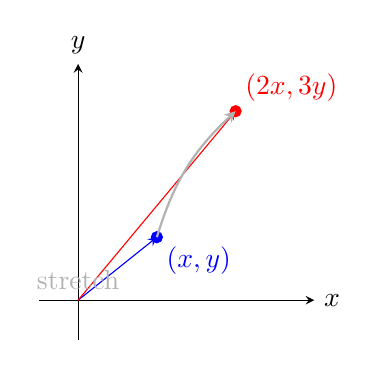
\begin{tikzpicture}[>=stealth, scale=1]
      % Axes
      \draw[->] (-0.5,0) -- (3,0) node[right] {$x$};
      \draw[->] (0,-0.5) -- (0,3) node[above] {$y$};
    
      % Original point P = (x,y)
      \coordinate (P) at (1,0.8);
      \filldraw[blue] (P) circle (2pt) node[below right] {$(x,y)$};
      \draw[blue,->] (0,0) -- (P);
    
      % Transformed point P' = (2x,3y)
      \coordinate (Pp) at (2*1,3*0.8);
      \filldraw[red] (Pp) circle (2pt) node[above right] {$(2x,3y)$};
      \draw[red,->] (0,0) -- (Pp);
    
      % Arrow showing mapping
      \draw[thick,->,gray!60] (P) to[bend left=15] (Pp) node[midway,above,sloped] {stretch};
    
    \end{tikzpicture}
    \caption{Original point $(x,y)$ (blue) is mapped to $(2x,3y)$ (red) by stretching $x$ by 2 and $y$ by 3.}
\end{figure}


\medskip
\noindent\textbf{2. Combining Two Operations}

Next, imagine you first stretch by \((2,3)\) and then rotate by \(90^\circ\).  Written out,
\[
\text{Stretch:}\quad (x,y)\;\mapsto\;(2x,\,3y),
\]
\[
\text{Rotate:}\quad (u,v)\;\mapsto\;(-v,\,u).
\]
Putting them together,
\[
(x,y)\;\mapsto\;(2x,3y)\;\mapsto\;(-3y,\,2x).
\]
Doing this repeatedly soon becomes tedious if you write each step by a separate formula.


\begin{figure}[H]
    \centering
    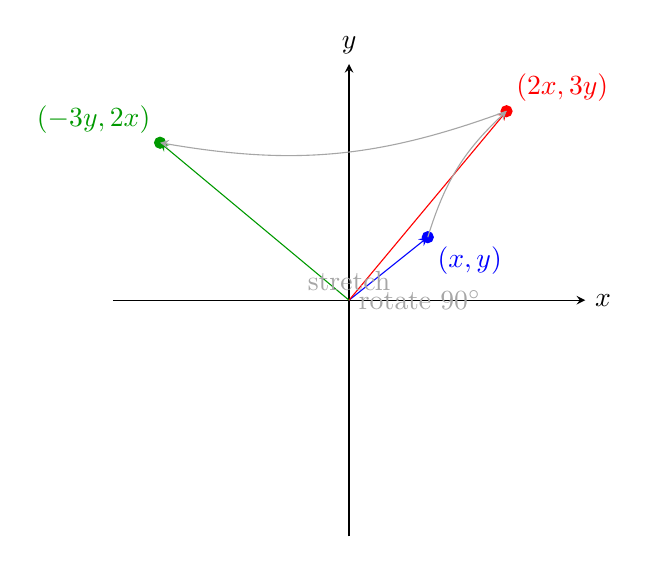
\begin{tikzpicture}[>=stealth,scale=1]
      % Axes
      \draw[->] (-3,0) -- (3,0) node[right] {$x$};
      \draw[->] (0,-3) -- (0,3) node[above] {$y$};
    
      % Original point P = (x,y)
      \coordinate (P) at (1,0.8);
      \filldraw[blue] (P) circle (2pt) node[below right] {$(x,y)$};
      \draw[blue,->] (0,0) -- (P);
    
      % After stretch S = (2x,3y)
      \coordinate (S) at (2*1,3*0.8); % (2,2.4)
      \filldraw[red] (S) circle (2pt) node[above right] {$(2x,3y)$};
      \draw[red,->] (0,0) -- (S);
    
      % After rotation R = (-3y,2x) = (-2.4,2)
      \coordinate (R) at (-2.4,2);
      \filldraw[green!60!black] (R) circle (2pt) node[above left] {$(-3y,2x)$};
      \draw[green!60!black,->] (0,0) -- (R);
    
      % Mapping arrows
      \draw[->,gray!70] (P) to[bend left=15] (S) node[midway,above] {stretch};
      \draw[->,gray!70] (S) to[bend left=15] (R) node[midway,right] {rotate $90^\circ$};
    
    \end{tikzpicture}
    \caption{Starting from $(x,y)$ (blue), first stretch to $(2x,3y)$ (red), then rotate by $90^\circ$ to $(-3y,2x)$ (green).}
    \end{figure}
    
    





\medskip
\noindent\textbf{3. Capturing All Coefficients in a Table}

Notice each linear step has the form
\[
\begin{cases}
u = a\,x + b\,y,\\
v = c\,x + d\,y,
\end{cases}
\]
where for the stretch \((a,b,c,d)=(2,0,0,3)\), and for the \(90^\circ\) rotation \((a,b,c,d)=(0,-1,1,0)\).  We can record these four numbers in a neat \(2\times2\) “box”:
\[
\begin{pmatrix}
a & b\\
c & d
\end{pmatrix}.
\]
This box of numbers is what Cayley named a \emph{matrix}.  The rule
\[
\begin{pmatrix}a&b\\c&d\end{pmatrix}
\begin{pmatrix}x\\y\end{pmatrix}
=
\begin{pmatrix}
a\,x + b\,y\\
c\,x + d\,y
\end{pmatrix}
\]
lets us apply the same table to any point \((x,y)\).

\begin{figure}[H]
    \centering
    \begin{tikzpicture}[>=stealth, node distance=1cm, every node/.style={font=\small}]
      % Matrix box
      \matrix (M) [matrix of math nodes,
                   left delimiter=(, right delimiter=),
                   nodes={minimum size=6mm, anchor=center}] {
        a & b \\
        c & d \\
      };
      \node[below=0.2cm of M] {Matrix $A$};
    
      % Multiply sign
      \node[right=of M] (times) {$\times$};
    
      % Input vector
      \matrix (X) [matrix of math nodes,
                   left delimiter=(, right delimiter=),
                   nodes={minimum size=6mm}] at ($(times)+(1.5cm,0)$) {
        x \\ y \\
      };
      \node[below=0.2cm of X] {Vector $(x,y)^\mathsf{T}$};
    
      % Equals sign
      \node[right=of X] (eq) {$=$};
    
      % Output vector
      \matrix (U) [matrix of math nodes,
                   left delimiter=(, right delimiter=),
                   nodes={minimum size=6mm}] at ($(eq)+(1.5cm,0)$) {
        u \\ v \\
      };
      \node[below=0.2cm of U] {Vector $(u,v)^\mathsf{T}$};
    
      % Equations u, v
      \node[below=1cm of eq, align=left] {
        $u = a\,x + b\,y$,\\
        $v = c\,x + d\,y$.
      };
    \end{tikzpicture}
    \caption{A $2\times2$ matrix $A=\bigl(\begin{smallmatrix}a&b\\c&d\end{smallmatrix}\bigr)$ acting on the column vector $(x,y)^\mathsf{T}$ produces $(u,v)^\mathsf{T}$ via $u=ax+by$ and $v=cx+dy$.}
\end{figure}





\medskip
\noindent\textbf{4. Chaining Operations by Multiplying Tables}

If you have one matrix \(A\) for stretching and another \(R\) for rotation, doing the stretch then the rotation is just
\[
R\bigl(A(x,y)\bigr)
=
\bigl(R\,A\bigr)\,(x,y)
\quad\Longrightarrow\quad
\text{compose transforms}\;\sim\;\text{multiply matrices }R\,A.
\]
This builds up more complicated motions by a single algebraic rule.


\begin{figure}[H]
    \centering
    \begin{tikzpicture}[>=stealth, node distance=1cm, every node/.style={font=\small}]
      % Matrix A: Stretch
      \node (MA) [matrix of math nodes,
                   left delimiter=(, right delimiter=),
                   nodes={minimum size=6mm}] {
        2 & 0 \\
        0 & 3 \\
      };
      \node[below=0.2cm of MA] {Stretch $A$};
    
      % Multiplication sign
      \node (times1) [right=of MA] {$\times$};
    
      % Matrix R: Rotate
      \node (MR) [matrix of math nodes,
                   left delimiter=(, right delimiter=),
                   nodes={minimum size=6mm}] at ($(times1)+(1.5cm,0)$) {
        0 & -1 \\
        1 & 0 \\
      };
      \node[below=0.2cm of MR] {Rotate $R$};
    
      % Equals sign
      \node (eq) [right=of MR] {$=$};
    
      % Composite matrix R A
      \node (MRA) [matrix of math nodes,
                    left delimiter=(, right delimiter=),
                    nodes={minimum size=6mm}] at ($(eq)+(1.5cm,0)$) {
        0 & -3 \\
        2 & 0 \\
      };
      \node[below=0.2cm of MRA] {Compose $R\,A$};
    
    \end{tikzpicture}
    \caption{Chaining transformations by matrix multiplication: stretching by $A$ then rotating by $R$ is achieved by applying the composite matrix $R\,A$.}
\end{figure}






\bigskip
\noindent\textbf{5. Measuring Area with the Determinant}

Cayley showed that a special “determinant” of the matrix
\(\begin{pmatrix}a&b\\c&d\end{pmatrix}\)
exactly measures how much a small area is scaled:
\[
\det
\begin{pmatrix}a&b\\c&d\end{pmatrix}
= ad - bc.
\]
For our stretch \(\bigl(\begin{smallmatrix}2&0\\0&3\end{smallmatrix}\bigr)\), we get \(2\times3-0=6\): the unit square becomes area 6.  For a rotation \(\bigl(\begin{smallmatrix}0&-1\\1&0\end{smallmatrix}\bigr)\), \(\det=1\): areas are preserved.


\begin{figure}[H]
    \centering
    \begin{subfigure}[b]{0.8\textwidth}
      \centering
      \begin{tikzpicture}[>=stealth, scale=1]
        % Axes
        \draw[->] (-0.5,0) -- (3,0) node[right] {$x$};
        \draw[->] (0,-0.5) -- (0,3) node[above] {$y$};
    
        % Original unit square
        \draw[thick,blue] (0,0) -- (1,0) -- (1,1) -- (0,1) -- cycle;
        \node[blue] at (0.7,0.3) {unit square};
    
        % Transformed parallelogram under S = [2 0; 0 3]
        \coordinate (v1) at (2,0);    % (a,c) = (2,0)
        \coordinate (v2) at (0,3);    % (b,d) = (0,3)
        \draw[fill=blue!20,opacity=0.5] (0,0) -- (v1) -- ($(v1)+(v2)$) -- (v2) -- cycle;
        \draw[->,red] (0,0) -- (v1) node[midway, below] {$(2,0)$};
        \draw[->,red] (0,0) -- (v2) node[midway, left] {$(0,3)$};
        \node at (1.5,1.8) {det\,$=2\cdot3 - 0 = 6$};
    
      \end{tikzpicture}
      \caption{Stretch by $\bigl(\begin{smallmatrix}2&0\\0&3\end{smallmatrix}\bigr)$ scales area by $\det=6$.}
    \end{subfigure}
    
    \vspace{1em}
    
    \begin{subfigure}[b]{0.8\textwidth}
      \centering
      \begin{tikzpicture}[>=stealth, scale=1]
        % Axes
        \draw[->] (-1.5,0) -- (1.5,0) node[right] {$x$};
        \draw[->] (0,-1.5) -- (0,1.5) node[above] {$y$};
    
        % Original unit square
        \draw[thick,blue] (0,0) -- (1,0) -- (1,1) -- (0,1) -- cycle;
        \node[blue] at (0.7,0.3) {unit square};
    
        % Transformed parallelogram under R = [0 -1; 1 0]
        \coordinate (u1) at (0,1);    % (a,c) = (0,1)
        \coordinate (u2) at (-1,0);   % (b,d) = (-1,0)
        \draw[fill=green!20,opacity=0.5] (0,0) -- (u1) -- ($(u1)+(u2)$) -- (u2) -- cycle;
        \draw[->,red] (0,0) -- (u1) node[midway, left] {$(0,1)$};
        \draw[->,red] (0,0) -- (u2) node[midway, below] {$(-1,0)$};
        \node at (-0.7,0.7) {det\,$=0\cdot0 - 1\cdot(-1) = 1$};
    
      \end{tikzpicture}
      \caption{Rotate by $\bigl(\begin{smallmatrix}0&-1\\1&0\end{smallmatrix}\bigr)$ preserves area ($\det=1$).}
    \end{subfigure}
    
    \caption{The determinant of a $2\times2$ matrix measures how it scales area: top, a stretch with $\det=6$; bottom, a $90^\circ$ rotation with $\det=1$.}
\end{figure}








\bigskip
\noindent\textbf{6. From Two to Many Dimensions}

Everything above carries over to \(n\) coordinates.  A general linear transform in \(\mathbb{R}^n\) is described by an \(n\times n\) matrix, and its determinant tells you how \(n\)-dimensional volume changes.  Cayley’s genius was to see that these tables of numbers—and the algebra of multiplying them and taking determinants—gave a unified language for all of geometry:

\begin{itemize}
  \item \emph{Rotations, reflections, shears, scalings} all become single matrices.
  \item \emph{Composition of motions} becomes matrix multiplication.
  \item \emph{Area or volume preservation} is precisely the condition \(\det=1\).
\end{itemize}

With this scaffold in place, one can revisit Jacobi’s action surfaces and see that any allowable change of coordinates in the Hamilton–Jacobi equation must come from a matrix of determinant one—ensuring the geometric “shape” of the surface (and the areas that embody Kepler’s Second Law) remains intact.


\begin{figure}[H]
    \centering
    \begin{tikzpicture}[>=stealth,scale=1]
      % Define a simple 3D projection basis
      \coordinate (O)  at (0,0);
      \coordinate (e)  at (1,0);     % x‐axis
      \coordinate (f)  at (0.3,0.6); % y‐axis
      \coordinate (g)  at (0,1.2);   % z‐axis
    
      % Draw the basis directions
      \draw[->] (O) -- (e) node[below right] {$(1,0,0)$};
      \draw[->] (O) -- (f) node[left]        {$(0,1,0)$};
      \draw[->] (O) -- (g) node[above]       {$(0,0,1)$};
    
      % Unit cube edges
      \draw (O) -- (e) -- ($(e)+(f)$) -- (f) -- cycle;
      \draw (O) -- (g) -- ($(g)+(e)$) -- (e) -- cycle;
      \draw (f) -- ($(f)+(g)$) -- ($(f)+(g)+(e)$) -- ($(f)+(e)$) -- cycle;
      \draw[dashed] (g) -- ($(g)+(f)$) -- ($(g)+(f)+(e)$);
    
      \node at ($(O)!0.5!(e)+(0.3,0.5)$) {Unit cube (vol = 1)};
    
      % Parallelepiped under M = diag(2,3,1)
      \begin{scope}[xshift=5cm]
        \coordinate (O2) at (0,0);
        \coordinate (e2) at (2,0);              % 2×e
        \coordinate (f2) at (0.9,1.8);          % 3×f
        \coordinate (g2) at (0,1.2);            % 1×g
    
        % Draw transformed axes
        \draw[->] (O2) -- (e2) node[below right] {$(2,0,0)$};
        \draw[->] (O2) -- (f2) node[left]        {$(0,3,0)$};
        \draw[->] (O2) -- (g2) node[above]       {$(0,0,1)$};
    
        % Parallelepiped edges
        \draw (O2) -- (e2) -- ($(e2)+(f2)$) -- (f2) -- cycle;
        \draw (O2) -- (g2) -- ($(g2)+(e2)$) -- (e2) -- cycle;
        \draw (f2) -- ($(f2)+(g2)$) -- ($(f2)+(g2)+(e2)$) -- ($(f2)+(e2)$) -- cycle;
        \draw[dashed] (g2) -- ($(g2)+(f2)$) -- ($(g2)+(f2)+(e2)$);
    
        \node at ($(O2)!0.5!(e2)+(0.3,0.5)$) {Parallelepiped (vol = $\det=6$)};
      \end{scope}
    
    \end{tikzpicture}
    \caption{Left: the unit cube in \(\mathbb{R}^3\), volume 1.  
    Right: its image under the diagonal matrix \(\mathrm{diag}(2,3,1)\), a parallelepiped of volume \(\det=2\cdot3\cdot1=6\).}
\end{figure}









\subsection{A Gentle Dive into Jacobians and Area Preservation}

So far we have seen that Cayley’s determinant tells us when a change of coordinates leaves Jacobi’s action surfaces—and the areas upon them—exactly unchanged.  Let us now unpack the key ideas in a bit more detail, but without losing sight of the geometric picture.

\textbf{1. From Small Squares to Parallelograms}

Imagine drawing a tiny square in your \((q,p)\) plane, with corners at
\[
(q,p),\quad (q+\delta q,p),\quad (q,p+\delta p),\quad (q+\delta q,p+\delta p).
\]
Under a smooth change of variables to new coordinates
\[
Q = Q(q,p),\qquad P = P(q,p),
\]
that little square becomes a parallelogram.  The question is: by what factor does its area change?


\begin{figure}[H]
    \centering
    \begin{tikzpicture}[>=stealth,scale=1]
      % Original (q,p) axes and square
      \begin{scope}[shift={(-3,0)}]
        \draw[->] (-0.5,0) -- (2,0) node[right] {$q$};
        \draw[->] (0,-0.5) -- (0,2) node[above] {$p$};
        \draw[fill=blue!20] (0,0) rectangle (1,1);
        \node at (0.5,-0.3) {\small Square in $(q,p)$};
      \end{scope}
    
      % Mapping arrow
      \draw[->,thick] (-1,1.2) to[bend left] (1,1.2) node[midway,above] {\small map $(Q,P)=J(q,p)$};
    
      % Transformed (Q,P) axes and parallelogram
      \begin{scope}[shift={(3,0)}]
        \draw[->] (-0.5,0) -- (3,0) node[right] {$Q$};
        \draw[->] (0,-0.5) -- (0,3) node[above] {$P$};
        % Corners of parallelogram: J*(0,0), J*(1,0), J*(1,1), J*(0,1)
        \coordinate (A) at (0,0);
        \coordinate (B) at (1.5,0.2);
        \coordinate (C) at ($(B)+(0.5,1.2)$);
        \coordinate (D) at (0.5,1.2);
        \draw[fill=red!20] (A) -- (B) -- (C) -- (D) -- cycle;
        \node at (1,-0.3) {\small Parallelogram in $(Q,P)$};
      \end{scope}
    \end{tikzpicture}
    \caption{A tiny square in the $(q,p)$ plane is carried by the linear map $(Q,P)=J(q,p)$ into a parallelogram in the $(Q,P)$ plane; the determinant of $J$ gives the ratio of their areas.}
\end{figure}








\textbf{2. The Jacobian Matrix}

To first order in \(\delta q,\delta p\), the sides of the parallelogram are
\[
\bigl(\delta Q,\;0\bigr)
\quad\text{and}\quad
\bigl(0,\;\delta P\bigr),
\]
where
\[
\delta Q 
\;\approx\;
\frac{\partial Q}{\partial q}\,\delta q
\;+\;
\frac{\partial Q}{\partial p}\,\delta p,
\quad
\delta P 
\;\approx\;
\frac{\partial P}{\partial q}\,\delta q
\;+\;
\frac{\partial P}{\partial p}\,\delta p.
\]
These four partial derivatives form the \emph{Jacobian matrix}
\[
J
=
\begin{pmatrix}
\displaystyle \frac{\partial Q}{\partial q}
&\displaystyle \frac{\partial Q}{\partial p}\\[6pt]
\displaystyle \frac{\partial P}{\partial q}
&\displaystyle \frac{\partial P}{\partial p}
\end{pmatrix}.
\]

\begin{figure}[H]
    \centering
    \begin{tikzpicture}[>=stealth,scale=1]
      % Left: (q,p) axes and small square
      \begin{scope}[shift={(-3,0)}]
        \draw[->] (-0.5,0) -- (2,0) node[right] {$q$};
        \draw[->] (0,-0.5) -- (0,2) node[above] {$p$};
        % small square corners
        \draw[thick,blue,fill=blue!20] (0,0) rectangle (1,0.8);
        \node[blue] at (0.5,0.4) {square};
      \end{scope}
    
      % Arrow to indicate mapping
      \draw[->,thick] (-1.5,1.2) to[bend left] (1.5,1.2)
        node[midway,above] {\small linearization};
    
      % Right: (Q,P) axes and parallelogram
      \begin{scope}[shift={(3,0)}]
        \draw[->] (-0.5,0) -- (3,0) node[right] {$Q$};
        \draw[->] (0,-0.5) -- (0,3) node[above] {$P$};
        % approximate side vectors
        \coordinate (v1) at (1.2,0.3);  % (~∂Q/∂q·δq + ∂Q/∂p·δp, ...)
        \coordinate (v2) at (0.4,1);    % (..., ∂P/∂q·δq + ∂P/∂p·δp)
        % draw parallelogram
        \draw[thick,red,fill=red!20] (0,0) -- (v1) -- ($(v1)+(v2)$) -- (v2) -- cycle;
        % draw side arrows
        \draw[->,red] (0,0) -- (v1) node[midway,below right] {$\delta Q$};
        \draw[->,red] (0,0) -- (v2) node[midway,above left]  {$\delta P$};
        \node[red] at ($(v1)!0.5!(v2)+(0.3,0.2)$) {parallelogram};
      \end{scope}
    
      % Jacobian matrix below, using inline math
      \node at (0,-1.2) {\(\displaystyle
        J \;=\;
        \begin{pmatrix}
          \frac{\partial Q}{\partial q}
          & \frac{\partial Q}{\partial p} \\[8pt]
          \frac{\partial P}{\partial q}
          & \frac{\partial P}{\partial p}
        \end{pmatrix}
      \)};
    
    \end{tikzpicture}
    \caption{%
    (Left) A small square of side lengths \(\delta q,\delta p\) in the \((q,p)\) plane.
    (Right) Under the linear approximation \((Q,P)=J(q,p)\), the square maps to a parallelogram spanned by \(\delta Q\) and \(\delta P\), where \(\delta Q\approx Q_q\,\delta q + Q_p\,\delta p\) and \(\delta P\approx P_q\,\delta q + P_p\,\delta p\).  The Jacobian matrix \(J\) encodes these partial derivatives.
    }
\end{figure}
    









\textbf{3. Determinant = Area‐Ratio}

The area of the original square is \(\delta q\,\delta p\).  The area of the transformed parallelogram is
\[
\det(J)\,\delta q\,\delta p.
\]
Hence
\[
\det(J)
\;=\;
\frac{\text{area after}}{\text{area before}}.
\]
When \(\det(J)=1\), the change of variables \((q,p)\mapsto(Q,P)\) is \emph{area‐preserving}.


\begin{figure}[H]
    \centering
    \begin{tikzpicture}[>=stealth,scale=1]
      % Original (q,p) square
      \begin{scope}[shift={(-3,0)}]
        \draw[->] (-0.5,0) -- (2,0) node[right] {$q$};
        \draw[->] (0,-0.5) -- (0,2) node[above] {$p$};
        \draw[fill=blue!20,thick] (0,0) rectangle (1,0.8);
        % Side-length labels
        \draw[<->] (0,0.9) -- node[above] {$\delta q$} (1,0.9);
        \draw[<->] (-0.3,0) -- node[left]  {$\delta p$} (-0.3,0.8);
        \node at (0.5,0.4) {area = $\delta q\,\delta p$};
      \end{scope}
    
      % Arrow indicating mapping by Jacobian
      \draw[->,thick] (-1,1.2) to[bend left=15] (1,1.2) node[midway,above] {\small linear map $J$};
    
      % Transformed (Q,P) parallelogram
      \begin{scope}[shift={(3,0)}]
        \draw[->] (-0.5,0) -- (2,0) node[right] {$Q$};
        \draw[->] (0,-0.5) -- (0,2) node[above] {$P$};
        \coordinate (v1) at (1.2,0.3);
        \coordinate (v2) at (0.4,1);
        \draw[fill=red!20,thick] (0,0) -- (v1) -- ($(v1)+(v2)$) -- (v2) -- cycle;
        % Transformed side-vector labels
        \draw[<->] (v1) -- ++(0,0.3) node[above] {$\delta Q$};
        \draw[<->] (v2) -- ++(-0.3,0) node[left]  {$\delta P$};
        \node at ($(v1)!0.5!(v2)+(0.3,0.2)$) {area = $\det(J)\,\delta q\,\delta p$};
      \end{scope}
    
      % Determinant = area ratio
      \node at (0,-1.5) {\(\displaystyle
        \det(J)
        = \frac{\text{area after}}{\text{area before}}
      \)};
      \node at (0,-2) {\emph{Area--preserving if \(\det(J)=1\).}};
    \end{tikzpicture}
    \caption{A small square in the \((q,p)\) plane is carried by the linear map \(J\) into a parallelogram in the \((Q,P)\) plane.  The determinant \(\det(J)\) is exactly the ratio of their areas.}
\end{figure}








\textbf{4. Canonical Transformations}

In Hamilton–Jacobi theory we look for new variables \((Q,P)\) that simplify the action surface \(S\).  Cayley’s insight is that the only allowable changes—those that keep Jacobi’s equation in the same form—are exactly those with
\[
\det(J) \;=\; 1.
\]
Such transformations are called \emph{canonical}: they preserve the “signed volume” (area in 2D, volume in higher dimensions) in phase space, and thus leave the geometry of \(S\) untouched.


\begin{figure}[H]
    \centering
    \begin{tikzpicture}[>=stealth,scale=1]
      % Original (q,p) axes and square
      \begin{scope}
        \draw[->] (-0.5,0) -- (2,0) node[right] {$q$};
        \draw[->] (0,-0.5) -- (0,2) node[above] {$p$};
        % small square
        \draw[thick,blue,fill=blue!20] (0,0) rectangle (1,1);
        % side labels
        \draw[<->] (0,1.1) -- node[above] {$\delta q$} (1,1.1);
        \draw[<->] (-0.1,0) -- node[left]  {$\delta p$} (-0.1,1);
        \node[blue] at (0.5,0.5) {square};
      \end{scope}
    
      % mapping arrow
      \draw[->,thick] (1.2,1.5) to[bend left=15] (3,1.5) node[midway,above] {\small canonical $J$};
    
      % Transformed (Q,P) axes and parallelogram
      \begin{scope}[xshift=4cm]
        \draw[->] (-0.5,0) -- (2,0) node[right] {$Q$};
        \draw[->] (0,-0.5) -- (0,2) node[above] {$P$};
        % shear J = [1 1; 0 1]
        \coordinate (A) at (0,0);
        \coordinate (B) at (1,0);
        \coordinate (D) at (0,1);
        \coordinate (C) at ($(B)+(D)$); % (1,1)
        % parallelogram
        \draw[thick,blue,fill=blue!20] (A) -- (B) -- (C) -- (D) -- cycle;
        % side labels
        \draw[<->] (0,1.1) -- node[above] {$\delta Q$} (1,1.1);
        \draw[<->] (-0.1,0) -- node[left]  {$\delta P$} (-0.1,1);
        \node[blue] at (0.8,0.5) {parallelogram};
        % determinant note
        \node at (1,-0.3) {$\det(J)=1$};
      \end{scope}
    \end{tikzpicture}
    \caption{A canonical transformation $J$ with \(\det(J)=1\) maps a small square of area \(\delta q\,\delta p\) in the \((q,p)\) plane to a parallelogram of the same area in the \((Q,P)\) plane, thus preserving the geometry of the action surface \(S\).}
\end{figure}








\textbf{5. A Simple Example: Rotation in the Plane}

As a concrete illustration, consider the rotation by angle \(\phi\):
\[
Q = q\cos\phi \;-\; p\sin\phi,
\quad
P = q\sin\phi \;+\; p\cos\phi.
\]
Here
\[
\frac{\partial(Q,P)}{\partial(q,p)}
=
\det
\begin{pmatrix}
\cos\phi & -\sin\phi\\[6pt]
\sin\phi & \cos\phi
\end{pmatrix}
= \cos^2\phi + \sin^2\phi = 1.
\]
Because the determinant is 1, this rotation is canonical—it simply “spins” the action surface without stretching or squeezing it.


\begin{figure}[H]
    \centering
    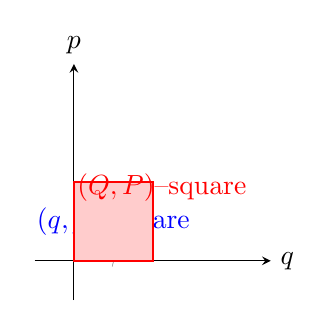
\begin{tikzpicture}[>=stealth,scale=1]
      % Axes
      \draw[->] (-0.5,0) -- (2.5,0) node[right] {$q$};
      \draw[->] (0,-0.5) -- (0,2.5) node[above] {$p$};
    
      % Original unit square in (q,p)
      \coordinate (A) at (0,0);
      \coordinate (B) at (1,0);
      \coordinate (C) at (1,1);
      \coordinate (D) at (0,1);
      \draw[thick,blue,fill=blue!20] (A) -- (B) -- (C) -- (D) -- cycle;
      \node[blue] at (0.5,0.5) {$(q,p)$–square};
    
      % Rotation angle arc
      \draw[->,gray] (0.3,0) arc[start angle=0,end angle=30,radius=0.3] 
        node[midway, right] {$\phi$};
    
      % Rotated square
      \begin{scope}[rotate=30]
        \draw[thick,red,fill=red!20] (A) -- (B) -- (C) -- (D) -- cycle;
      \end{scope}
      \node[red] at ({cos(30)+0.5*sin(30)},{sin(30)+0.5*cos(30)}) {$(Q,P)$–square};
    
    \end{tikzpicture}
    \caption{A unit square in the $(q,p)$ plane (blue) rotated by angle $\phi$ about the origin (gray arc) becomes a congruent square (red) in the $(Q,P)$ plane.  Since $\det R(\phi)=1$, the area is preserved.}
\end{figure}





\textbf{6. Why This Matters}

By insisting on \(\det(J)=1\), Cayley’s approach guarantees that every small patch of Jacobi’s landscape has the same shape before and after a coordinate change.  This algebraic criterion underlies the stability of the Hamilton–Jacobi equation under re‐labeling of coordinates, and it ties back directly to Kepler’s Second Law via the area‐preserving property of rotations in phase space.




\subsection{Determinants as Invariants of Jacobi’s Surfaces}

Jacobi showed us that all motions lie on level‐surfaces of a single function \(S(q,t)\).  Cayley went further: he asked how those surfaces themselves change when we switch from one set of coordinates to another.  The answer lay in a simple algebraic expression—the \emph{determinant} of the Jacobian matrix of the transformation.

\textbf{1. Change of Coordinates and the Jacobian.}  

Suppose we replace generalized coordinates \(q_i\) by new variables \(Q_i = Q_i(q)\).  The effect on the surface \(S(q,t)\) is governed by the matrix

\[
\frac{\partial Q}{\partial q}
\;=\;
\biggl[\frac{\partial Q_i}{\partial q_j}\biggr]_{i,j},
\]

and the determinant

\[
\det\!\biggl(\frac{\partial Q}{\partial q}\biggr)
\]

measures exactly how infinitesimal volume (or “area” in two dimensions) on the surface is distorted.  If this determinant equals 1, the surface’s local geometry—and hence the form of Jacobi’s equation—remains unchanged.


\begin{figure}[H]
    \centering
    \begin{tikzpicture}[>=stealth,scale=1]
    
      % Left: original q‐grid and square patch
      \begin{scope}[shift={(-3,0)}]
        \draw[->] (-0.5,0) -- (2,0) node[right] {$q_1$};
        \draw[->] (0,-0.5) -- (0,2) node[above] {$q_2$};
        % grid
        \foreach \x in {0,1,2} \draw (\x,0) -- (\x,2);
        \foreach \y in {0,1,2} \draw (0,\y) -- (2,\y);
        % highlighted square
        \draw[fill=blue!20,thick] (0,0) rectangle (1,1);
        \node[blue] at (0.5,0.5) {patch};
      \end{scope}
    
      % arrow mapping
      \draw[->,thick] (-1.5,1.5) to[bend left] (1.5,1.5) node[midway,above] {\small linear map \(J\)};
    
      % Right: transformed Q‐grid and parallelogram patch
      \begin{scope}[shift={(3,0)}]
        \draw[->] (-0.5,0) -- (3,0) node[right] {$Q_1$};
        \draw[->] (0,-0.5) -- (0,3) node[above] {$Q_2$};
    
        % Images of basis vectors under J
        \coordinate (e1) at (1.5,0.2);  % J*(1,0)
        \coordinate (e2) at (0.3,1.3);  % J*(0,1)
        \draw[->] (0,0) -- (e1) node[below right]
          {\(\bigl(\partial Q_1/\partial q_1,\partial Q_2/\partial q_1\bigr)\)};
        \draw[->] (0,0) -- (e2) node[above left]
          {\(\bigl(\partial Q_1/\partial q_2,\partial Q_2/\partial q_2\bigr)\)};
    
        % highlighted parallelogram
        \draw[fill=red!20,thick] (0,0) -- (e1) -- ($(e1)+(e2)$) -- (e2) -- cycle;
        \node[red] at ($(e1)!0.5!(e2)+(0.2,0.2)$) {patch};
      \end{scope}
    
      % Jacobian determinant ratio below
      \node at (0,-1.5) {\(\displaystyle
        J = \begin{pmatrix}
          \frac{\partial Q_1}{\partial q_1} & \frac{\partial Q_1}{\partial q_2}\\[6pt]
          \frac{\partial Q_2}{\partial q_1} & \frac{\partial Q_2}{\partial q_2}
        \end{pmatrix}
        ,\quad
        \det J = \frac{\text{area of red patch}}{\text{area of blue patch}}.
      \)};
    
    \end{tikzpicture}
    \caption{Under the change of coordinates \((q_1,q_2)\mapsto(Q_1,Q_2)\), a unit square in the \((q_1,q_2)\) plane (blue) is carried by the linear approximation \(J\) into a parallelogram in the \((Q_1,Q_2)\) plane (red).  The determinant \(\det J\) gives the ratio of their areas.}
\end{figure}
    












\textbf{2. Canonical Transformations.}  
In Hamilton–Jacobi theory one often seeks new variables \((Q,P)\) in which the action surface \(S\) takes a simpler form.  Cayley’s determinant gives the criterion:

\[
\det
\begin{pmatrix}
\displaystyle \frac{\partial Q}{\partial q} & \displaystyle \frac{\partial Q}{\partial p}\\[8pt]
\displaystyle \frac{\partial P}{\partial q} & \displaystyle \frac{\partial P}{\partial p}
\end{pmatrix}
\;=\;1
\]

ensures that the new surface preserves the “signed volume” in \((q,p)\)–space.  Such transformations—now called \emph{canonical}—leave Jacobi’s equation invariant.


\begin{figure}[H]
    \centering
    \begin{tikzpicture}[>=stealth,scale=1]
      % Left: (q,p) axes and unit square
      \begin{scope}
        \draw[->] (-0.5,0) -- (2,0) node[right] {$q$};
        \draw[->] (0,-0.5) -- (0,2) node[above] {$p$};
        \draw[thick,blue,fill=blue!20] (0,0) rectangle (1,1);
        \node[blue] at (0.5,0.5) {unit square};
      \end{scope}
    
      % Label det=1 above arrow
      \node at (2.5,1.5) {\(\det(J)=1\)};
    
      % Arrow mapping
      \draw[->,thick] (1.1,0.8) to[bend left] (2.9,0.8) node[midway,above] {\small canonical \(J\)};
    
      % Right: (Q,P) axes and parallelogram
      \begin{scope}[xshift=5cm]
        \draw[->] (-0.5,0) -- (2,0) node[right] {$Q$};
        \draw[->] (0,-0.5) -- (0,2) node[above] {$P$};
        % Basis images for canonical J (e.g.\ shear with det=1)
        \coordinate (e1) at (1.2,0.3);
        \coordinate (e2) at (0.4,1);
        \draw[thick,red,fill=red!20] (0,0) -- (e1) -- ($(e1)+(e2)$) -- (e2) -- cycle;
        \node[red] at ($(e1)!0.5!(e2)+(0.2,0.2)$) {parallelogram};
      \end{scope}
    
    \end{tikzpicture}
    \caption{A canonical transformation \(J\) with \(\det(J)=1\) carries a unit square in the \((q,p)\) plane (blue) into a parallelogram of equal area in the \((Q,P)\) plane (red), thus preserving the local “signed volume” of Jacobi’s action surface.}
\end{figure}





\textbf{3. Linearization and Local Analysis.}  
By linearizing a nonlinear coordinate change near a point on the surface, Cayley’s determinant tells us whether the local shape of \(S\) is preserved (unit determinant), squeezed (\(<1\)), or stretched (\(>1\)).  This insight allows one to classify equilibrium points and to understand the stability of trajectories by purely algebraic means.


\begin{figure}[H]
    \centering
    \begin{tikzpicture}[>=stealth,scale=1]
    
      % det < 1: Squeezing
      \begin{scope}[shift={(-4,0)}]
        % axes
        \draw[->] (-0.5,0) -- (1.5,0) node[right] {};
        \draw[->] (0,-0.5) -- (0,1.5) node[above] {};
        % original square
        \draw[thick,blue,fill=blue!20] (0,0) rectangle (1,1);
        % linear map J1
        \draw[->,gray!70] (0.5,1.2) -- ++(1,0) node[midway,above] {\(\det J<1\)};
        % squeezed parallelogram
        \coordinate (u1) at (0.8,0.2);
        \coordinate (u2) at (0.1,0.8);
        \draw[thick,red,fill=red!20] (0,0) -- (u1) -- ($(u1)+(u2)$) -- (u2) -- cycle;
        \node[red] at (0.4,0.4) {squeezed};
      \end{scope}
    
      % det = 1: Preserving
      \begin{scope}[shift={(0,0)}]
        \draw[->] (-0.5,0) -- (1.5,0) node[right] {};
        \draw[->] (0,-0.5) -- (0,1.5) node[above] {};
        \draw[thick,blue,fill=blue!20] (0,0) rectangle (1,1);
        \draw[->,gray!70] (0.5,1.2) -- ++(1,0) node[midway,above] {\(\det J=1\)};
        \coordinate (v1) at (1,0.2);
        \coordinate (v2) at (0.2,1);
        \draw[thick,green!60!black,fill=green!20] (0,0) -- (v1) -- ($(v1)+(v2)$) -- (v2) -- cycle;
        \node[green!60!black] at (0.6,0.6) {preserved};
      \end{scope}
    
      % det > 1: Stretching
      \begin{scope}[shift={(4,0)}]
        \draw[->] (-0.5,0) -- (1.5,0) node[right] {};
        \draw[->] (0,-0.5) -- (0,1.5) node[above] {};
        \draw[thick,blue,fill=blue!20] (0,0) rectangle (1,1);
        \draw[->,gray!70] (0.5,1.2) -- ++(1,0) node[midway,above] {\(\det J>1\)};
        \coordinate (w1) at (1.3,0.3);
        \coordinate (w2) at (0.3,1.3);
        \draw[thick,orange,fill=orange!20] (0,0) -- (w1) -- ($(w1)+(w2)$) -- (w2) -- cycle;
        \node[orange] at (0.8,0.8) {stretched};
      \end{scope}
    
    \end{tikzpicture}
    \caption{Local linearization of a nonlinear change of variables.  A unit square (blue) maps under \(J\) to a parallelogram (red/green/orange).  If \(\det J<1\), area is squeezed; if \(\det J=1\), area is preserved (canonical); if \(\det J>1\), area is stretched.}
\end{figure}






\textbf{4. From Surfaces to Structure.}  
Where Jacobi dealt with differential equations on a fixed backdrop of \(q\)-space, Cayley’s determinant turned the backdrop itself into an algebraic object.  Now the \emph{relations} among coordinates—their Jacobian determinants—became as important as the surfaces they parameterize.  In this way, the mechanics of surfaces yielded to the algebra of transformations, completing the passage from geometry to structure that underpins much of modern mathematical physics.  


\begin{figure}[H]
    \centering
    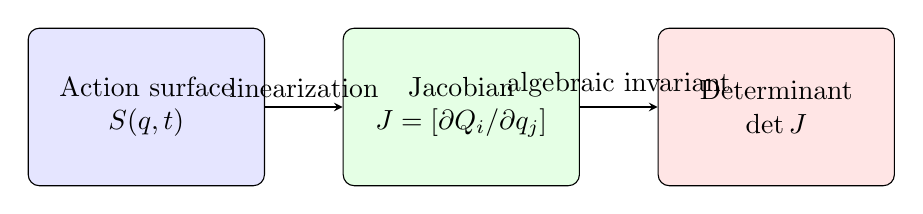
\begin{tikzpicture}[>=stealth, node distance=4cm, auto]
      % Surface block
      \node (surf) [draw, fill=blue!10, rounded corners, minimum width=3cm, minimum height=2cm, align=center]
        {Action surface\\\(S(q,t)\)};
    
      % Jacobian block
      \node (jac) [draw, fill=green!10, rounded corners, minimum width=3cm, minimum height=2cm, align=center, right of=surf]
        {Jacobian\\\(J = [\partial Q_i/\partial q_j]\)};
    
      % Determinant block
      \node (det) [draw, fill=red!10, rounded corners, minimum width=3cm, minimum height=2cm, align=center, right of=jac]
        {Determinant\\\(\det J\)};
    
      % Arrows
      \draw[->] (surf) -- node[above] {linearization} (jac);
      \draw[->] (jac)  -- node[above] {algebraic invariant} (det);
    \end{tikzpicture}
    \caption{From geometry to structure: a local patch of the action surface \(S(q,t)\) is linearized by its Jacobian \(J\), and the determinant \(\det J\) provides the invariant that encodes how the surface’s “volume” is preserved under coordinate changes.}
\end{figure}
    






\subsection{From Jacobi’s Surfaces to Cayley’s Algebra}

Where Jacobi invited us to explore the world by tracing level‐surfaces of a single function \(S(q,t)\), Cayley asked a different question: what algebraic structures underlie those surfaces themselves?  In this transition, three key shifts occur:

\textbf{Key Object}  

\begin{itemize}
    \item \emph{Jacobi:} The primary focus is the family of level sets
    \[
    S(q,t) = \text{constant},
    \]
    each of which encodes one possible trajectory.  These surfaces in the \((q,t)\) “configuration” space represent motion as geometry.  

    \item \emph{Cayley:} The fundamental entities become \emph{matrices}—arrays of numbers that capture how one coordinate system is carried into another.  Instead of studying individual surfaces, Cayley studies the transformations between coordinate patches.
\end{itemize}

\textbf{Geometry as...}  

\begin{itemize}
    \item \emph{Jacobi:} Surfaces embedded in a fixed backdrop of \(q\)–space.  Motion is read off by following the contours of \(S\).  
    \item \emph{Cayley:} Relations between coordinate systems themselves.  The shape of a surface becomes secondary to the \emph{algebra} of the maps that carry one set of axes into another—each map packaged neatly as a determinant‐carrying matrix.
\end{itemize}

\textbf{Equation Type}  
\begin{itemize}
    \item \emph{Jacobi:} A single partial differential equation (the Hamilton–Jacobi equation) whose solution \(S\) yields all trajectories at once.  
    \item \emph{Cayley:} Algebraic equations—the characteristic polynomials, determinants, and matrix products—that govern how these transformations combine and preserve geometric invariants.
\end{itemize}

\medskip
In moving from Jacobi to Cayley, mechanics shifts from “What surface does the system follow?” to “What algebraic rules govern changes of viewpoint?”  Surfaces give way to structure, and geometry is recast as the algebra of transformations.  







\subsection{Transforming Geometry Itself}

Cayley’s work foreshadowed a profound shift:

Geometry was no longer just the study of shapes, but the study of \textbf{invariants under transformation}.

Instead of focusing on points and lines, Cayley turned attention to the operations that moved, stretched, 
or rotated those objects,  and to the quantities that remained unchanged under such operations.

Where Jacobi had used surfaces to encode motion,  
Cayley showed that such surfaces could themselves be encoded in algebraic structures.

And while Jacobi’s equation governed how trajectories unfolded,  
Cayley’s matrices governed how spaces themselves were connected.


\begin{quote}
In Euler, we pushed.  
In Lagrange, we minimized.  
In Hamilton, we flowed.  
In Jacobi, we found surfaces.  
In Cayley, we discovered the algebra beneath those surfaces.
\end{quote}





\subsection{Kepler’s Second Law on an Elliptical Orbit}

Cayley’s determinant argument—namely that a small “rotation” about the focus has unit determinant and so preserves the area of any infinitesimal parallelogram—holds for \emph{any} central orbit, including ellipses.  In polar coordinates the area swept by the radius vector in a small angle \(\Delta\theta\) is
\[
\Delta A \;=\;\tfrac12\,r^2\,\Delta\theta.
\]
Because \(\det R(\Delta\theta)=1\) for the rotation matrix \(R(\Delta\theta)\), this formula is exact to first order in \(\Delta\theta\), regardless of how \(r\) varies with \(\theta\).  For an ellipse,
\[
r(\theta)
=\frac{a(1-e^2)}{1+e\cos\theta},
\]
the radius changes between perihelion and aphelion, but the combination \(r^2\,\Delta\theta\) remains the same for equal time intervals.  Concretely:

\begin{itemize}
    \item Near \textbf{perihelion}, \(r\) is small, so \(\Delta\theta\) must be larger to keep \(\tfrac12\,r^2\,\Delta\theta\) constant.
    \item Near \textbf{aphelion}, \(r\) is large, so \(\Delta\theta\) is correspondingly smaller.
\end{itemize}

\begin{figure}[H]
\centering
\begin{tikzpicture}[>=stealth, scale=1]
  % Draw a generic ellipse
  \draw[thick] (0,0) ellipse (2cm and 1cm);
  % Mark the focus
  \coordinate (F) at (-0.8,0);
  \fill (F) circle (2pt) node[below left]{Focus};

  % Perihelion wedge (blue): smaller radius, larger angle
  \draw[blue,thick] (F) -- ++(20:1.7cm) coordinate (P1);
  \draw[blue,thick] (F) -- ++(-40:1.7cm) coordinate (P2);
  \fill[blue!20] 
    (F) -- (P2) arc[start angle=-40,end angle=20,radius=1.7cm] -- cycle;
  \node[blue] at ($(F)+(0:1.2cm)+(90:0.3cm)$) {\(\Delta\theta_p\)};

  % Aphelion wedge (red): larger radius, smaller angle
  \draw[red,thick] (F) -- ++(150:2.9cm) coordinate (A1);
  \draw[red,thick] (F) -- ++(170:2.9cm) coordinate (A2);
  \fill[red!20] 
    (F) -- (A2) arc[start angle=170,end angle=150,radius=2.9cm] -- cycle;
  \node[red] at ($(F)+(160:2.1cm)+(270:0.3cm)$) {\(\Delta\theta_a\)};

  % Labels for points
  \node at ($(F)+(20:1.7cm)+(10:0.3cm)$) {perihelion};
  \node at ($(F)+(160:2.9cm)+(160:0.3cm)$) {aphelion};
\end{tikzpicture}
\caption{On an ellipse with focus \(F\), the blue wedge at perihelion (small \(r\)) spans a larger angle \(\Delta\theta_p\), while the red wedge at aphelion (large \(r\)) spans a smaller \(\Delta\theta_a\), yet both shaded areas satisfy \(\tfrac12\,r^2\,\Delta\theta=\) constant.  This geometric fact is a direct consequence of \(\det R(\Delta\theta)=1\) and underlies Kepler’s Second Law.}
\end{figure}


\subsection{Matrix Derivation of Kepler’s Areal Law}

To see Kepler’s Second Law emerge directly from matrix geometry, consider the infinitesimal rotation of the radius vector
\[
\mathbf{r} = \begin{pmatrix}x\\y\end{pmatrix}.
\]
A small change in angle \(\Delta\theta\) is effected by the rotation matrix
\[
R(\Delta\theta)
= I + \Delta\theta\,J + O(\Delta\theta^2),
\quad
J = \begin{pmatrix}0 & -1\\[4pt]1 & 0\end{pmatrix},
\]
whose determinant satisfies
\[
\det R(\Delta\theta)
= \det(I + \Delta\theta\,J)
= 1 + \Delta\theta\,\mathrm{tr}\,J + O(\Delta\theta^2)
= 1
\quad\text{(since } \mathrm{tr}\,J=0\text{).}
\]

Now the two vectors at times \(t\) and \(t+\Delta t\) are
\[
\mathbf{r}_1 = \mathbf{r}, 
\qquad
\mathbf{r}_2 = R(\Delta\theta)\,\mathbf{r} = \mathbf{r} + \Delta\theta\,J\,\mathbf{r}.
\]
The area of the parallelogram they span is
\[
\det\bigl[\mathbf{r}_1,\mathbf{r}_2\bigr]
= \det\bigl[\mathbf{r},\,\mathbf{r} + \Delta\theta\,J\,\mathbf{r}\bigr]
= \Delta\theta \;\det\bigl[\mathbf{r},\,J\,\mathbf{r}\bigr]
= \Delta\theta\,(x^2+y^2)
= \Delta\theta\,r^2.
\]
Hence the actual area swept is
\[
\Delta A \;=\;\tfrac12\,\det\bigl[\mathbf{r}_1,\mathbf{r}_2\bigr]
\;=\;\tfrac12\,r^2\,\Delta\theta.
\]

Since \(R(\Delta\theta)\) has \(\det=1\), this result is exact to first order and independent of the orbit’s shape.  In particular, for the ellipse
\[
r(\theta)
=\frac{a(1-e^2)}{1+e\cos\theta},
\]
the same derivation shows that equal increments \(\Delta\theta\) (and hence equal time intervals, because \(r^2\dot\theta\) is constant) sweep out equal areas \(\Delta A\).  Thus Kepler’s Second Law is nothing but the statement that infinitesimal rotations of unit determinant preserve the areal increments around the focus.


\begin{figure}[H]
    \centering
    % 1) Elliptical orbit with equal‐area wedges
    \begin{subfigure}[b]{0.45\textwidth}
      \centering
      \begin{tikzpicture}[>=stealth,scale=0.8]
        % Ellipse parameters
        \draw[thick,blue,domain=0:360,smooth,samples=200]
          plot ({(2.25/(1+0.5*cos(\x)))*cos(\x)},
               {(2.25/(1+0.5*cos(\x)))*sin(\x)});
        % Focus
        \coordinate (F) at (-0.8,0);
        \fill (F) circle (1.5pt) node[below left]{Focus};
    
        % Perihelion wedge (blue)
        \draw[blue,thick] (F) -- ++(20:1.7cm) coordinate (P1);
        \draw[blue,thick] (F) -- ++(-40:1.7cm) coordinate (P2);
        \fill[blue!20] 
          (F) -- (P2) arc[start angle=-40,end angle=20,radius=1.7cm] -- cycle;
        \node[blue] at ($(F)+(0:1.2cm)+(90:0.3cm)$){$\Delta\theta_p$};
    
        % Aphelion wedge (red)
        \draw[red,thick] (F) -- ++(150:2.9cm) coordinate (A1);
        \draw[red,thick] (F) -- ++(170:2.9cm) coordinate (A2);
        \fill[red!20] 
          (F) -- (A2) arc[start angle=170,end angle=150,radius=2.9cm] -- cycle;
        \node[red] at ($(F)+(160:2.1cm)+(270:0.3cm)$){$\Delta\theta_a$};
    
        % Labels
        \node at ($(F)+(20:1.7cm)+(10:0.3cm)$){perihelion};
        \node at ($(F)+(160:2.9cm)+(160:0.3cm)$){aphelion};
      \end{tikzpicture}
      \caption{Elliptical orbit: smaller $r$ (perihelion) gives larger $\Delta\theta_p$, larger $r$ (aphelion) gives smaller $\Delta\theta_a$, with $\tfrac12r^2\Delta\theta$ constant.}
    \end{subfigure}
    \quad
    % 2) Cayley's area‐preserving parallelogram
    \begin{subfigure}[b]{0.45\textwidth}
      \centering
      \begin{tikzpicture}[>=stealth,scale=1]
        % Origin
        \coordinate (O) at (0,0);
        % Radius vector r
        \coordinate (r) at (2,1);
        \draw[->,blue] (O) -- (r) node[midway,above right] {$\mathbf r$};
        % Infinitesimal rotation Jr (J=90° generator)
        \coordinate (Jr) at (-1,2);
        \draw[->,blue] (O) -- (Jr) node[midway,above left] {$J\,\mathbf r$};
    
        % Parallelogram spanned by r and Jr
        \draw[fill=blue!20,thick] (O) -- (r) -- ($(r)+(Jr)$) -- (Jr) -- cycle;
        \node at ($(O)!0.5!(r)+(0,0.5)$){$\displaystyle\det[\mathbf r,\;J\mathbf r]=r^2$};
      \end{tikzpicture}
      \caption{Cayley’s determinant: the infinitesimal rotation $J$ (with $\det=1$) carries $\mathbf r$ into $J\mathbf r$, and the parallelogram area $\det[\mathbf r,J\mathbf r]=r^2$ yields $\Delta A=\tfrac12r^2\Delta\theta$.}
    \end{subfigure}
    \caption{%
    Comparison of Kepler’s Second Law:  
    Left, the geometric wedge argument on the ellipse;  
    Right, Cayley’s matrix argument showing area preservation under an infinitesimal rotation with unit determinant.}
\end{figure}


\begin{figure}[H]
    \centering
    \begin{tikzpicture}[>=stealth, scale=1]
      % Coordinates
      \coordinate (O) at (0,0);
      \coordinate (R) at (2,1);                % \mathbf{r}
      \coordinate (dv) at (-0.3,0.6);          % \Delta\theta\,J\,\mathbf{r}
      \coordinate (R2) at ($(R)+(dv)$);        % \mathbf{r}_2 = \mathbf{r} + dv
    
      % Axes
      \draw[->] (-0.5,0) -- (3,0) node[right] {$x$};
      \draw[->] (0,-0.5) -- (0,2.5) node[above] {$y$};
    
      % Vectors
      \draw[->] (O) -- (R) node[pos=0.6, below right] {$\mathbf{r}$};
      \draw[->,green!60!black] (O) -- (R2) node[pos=0.6, above right] {$\mathbf{r}_2$};
      \draw[->,red,dashed] (O) -- (dv) node[pos=0.6, left] {$\Delta\theta\,J\mathbf{r}$};
    
      % Parallelogram shading
      \draw[fill=blue!20,draw=blue] (O) -- (R) -- (R2) -- (dv) -- cycle;
    
      % Area label
      \node at ($(O)!0.4!(R2)$) {\(\Delta A = \tfrac12\,\det[\mathbf{r},\,\mathbf{r}_2] = \tfrac12\,r^2\,\Delta\theta\)};
    
    \end{tikzpicture}
    \caption{The parallelogram spanned by \(\mathbf{r}\) and \(\Delta\theta\,J\mathbf{r}\) (dashed) has area \(\det[\mathbf{r},\Delta\theta\,J\mathbf{r}] = r^2\Delta\theta\), so \(\Delta A = \tfrac12\,r^2\,\Delta\theta\).  Since \(J\) generates a rotation of unit determinant, this geometric fact underlies Kepler’s Second Law on any orbit.}
\end{figure}

